\begin{frame}{AIs Keep Getting Better at Doing Research}
\begin{columns}[t]
\column{0.5\textwidth}
\centering
\textbf{Implementing experiments}

\vspace{0.4em}
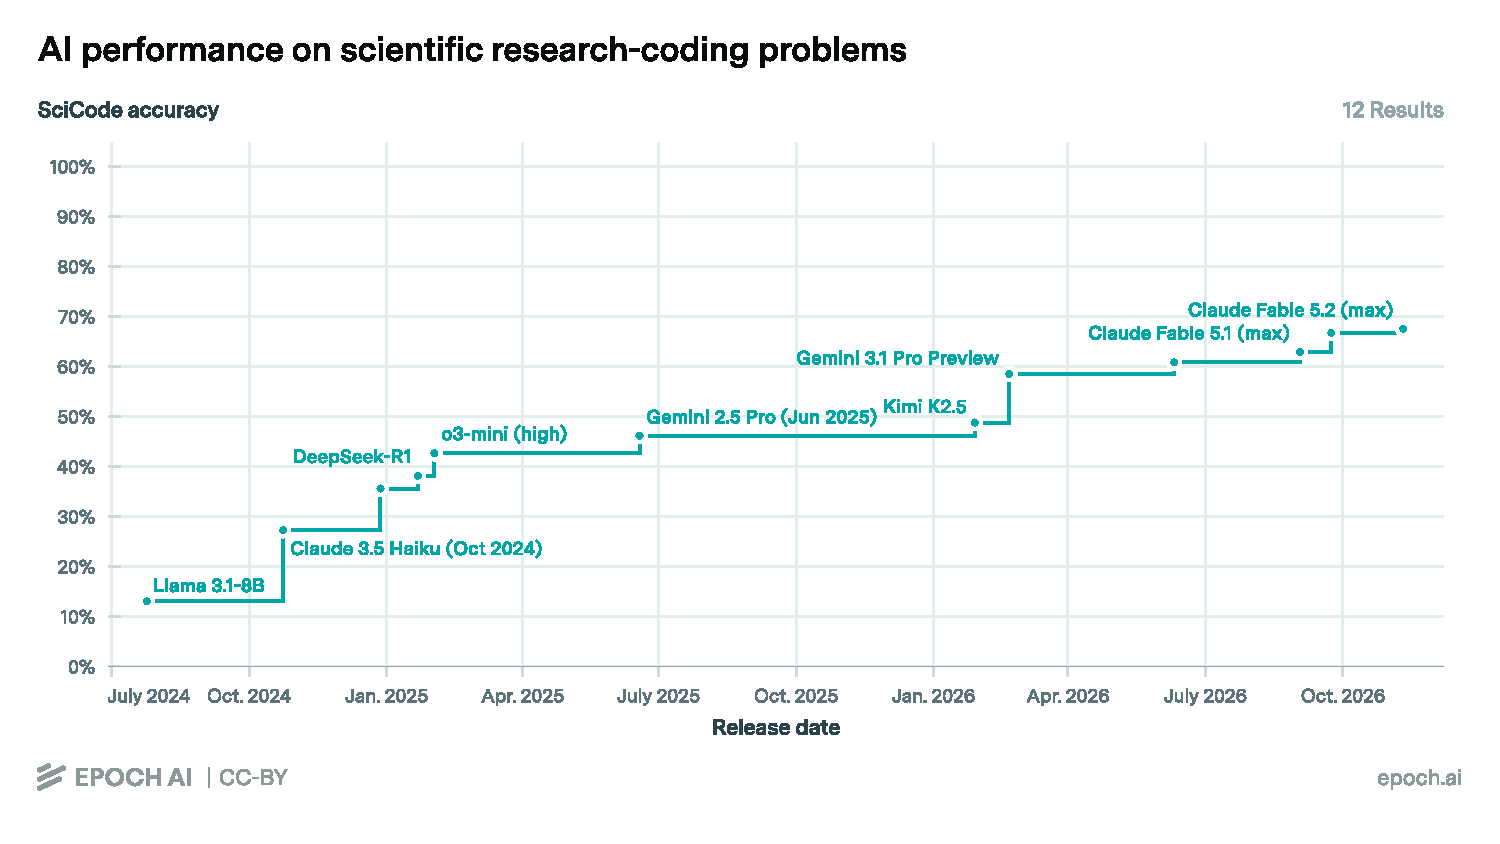
\includegraphics[width=\linewidth]{epoch_scicode_frontier}

{\small SciCode: research coding}
\column{0.5\textwidth}
\centering
\textbf{Choosing experiments}

\vspace{0.4em}
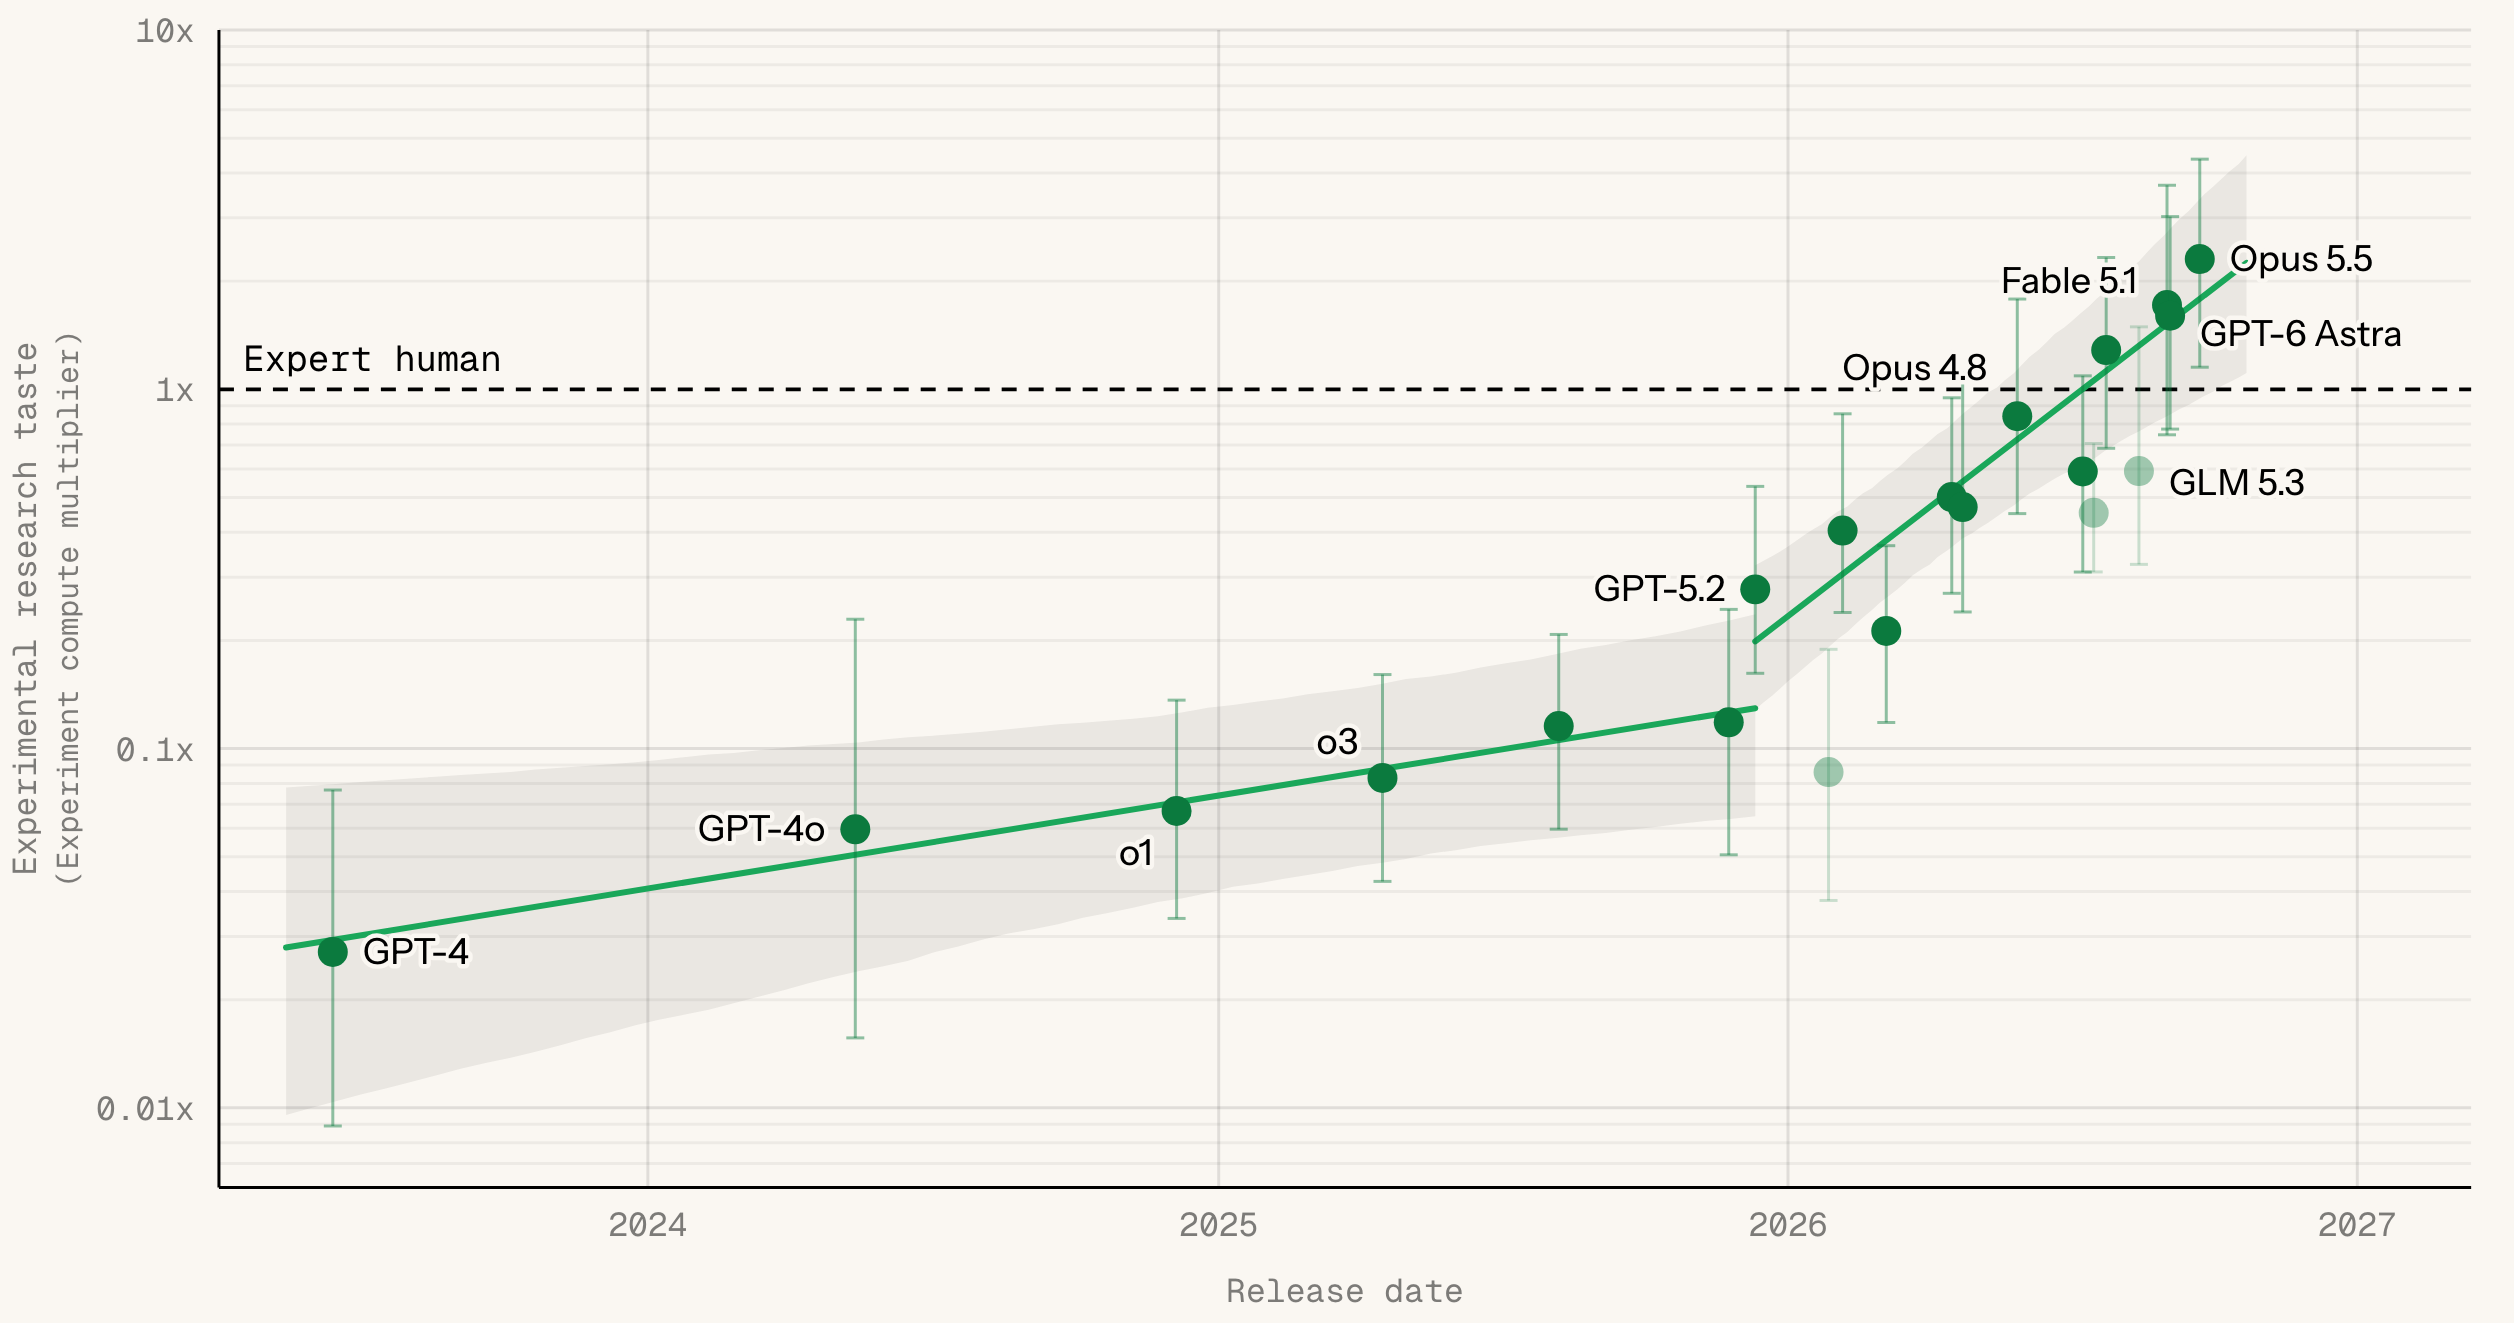
\includegraphics[width=\linewidth]{tasteval}

{\small TasteVal: research taste}
\end{columns}
\source{epochscicode2026,jaffe2026}
\end{frame}

\begin{frame}{Claude Already Does Much of the R\&D at Anthropic}
\centering
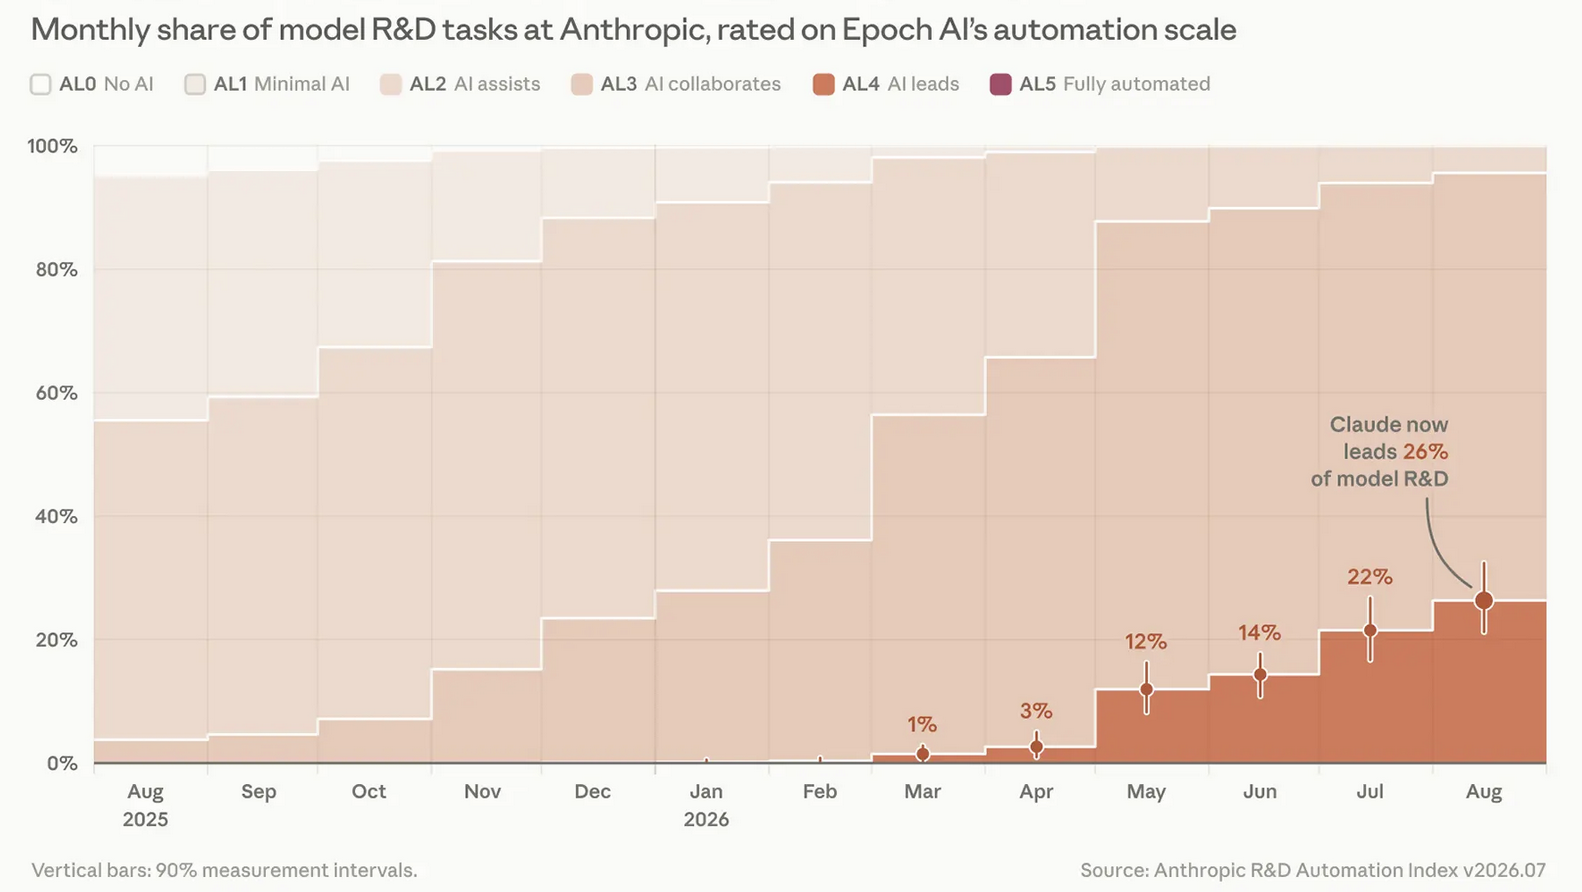
\includegraphics[height=0.72\textheight]{bib/zotero-item-1327/figures/auto_reserach_fraction}
\source{zotero-item-1327}
\end{frame}

\begin{frame}{METR: Evaluators Embedded at Anthropic}
\begin{columns}[t]
\column{0.5\textwidth}
\textbf{The assessment}
\begin{itemize}
\item 12 August to 29 October 2026: eleven weeks
\item 2.5 full-time METR staff
\item No payment in either direction
\item A $\sim$100-page full report for Anthropic, a redacted public report
\end{itemize}
\column{0.5\textwidth}
\textbf{What METR got to see}
\begin{itemize}
\item Benchmark scores of unreleased internal models
\item Algorithmic efficiency and training compute over time
\item Headcount, lines of code, AI agent spend
\item Internal surveys of AI uplift
\item $\sim$15 interviews with key staff
\end{itemize}
\end{columns}
\vspace{0.8em}
\centering
{\small Not employee-level access. Anthropic could redact anything non-public.}
\source{metr2026}
\end{frame}

\begin{frame}{METR: What Does ``Acceleration'' Mean?}
\textbf{Definition}

\vspace{0.3em}
A 2$\times$ acceleration means: two years of historical progress are made in one year.

\vspace{1.2em}
\pause
\textbf{METR's conclusion, October 2026}
\begin{itemize}
\item Anthropic is improving its models at about \textbf{2$\times$} the historical rate\\
{\small (they would not be surprised by anything from 1.3$\times$ to 3$\times$)}
\item A majority of this, perhaps \textbf{80\%}, is due to AI doing R\&D
\item No bottleneck in sight for the next 12 months
\end{itemize}
\source{metr2026}
\end{frame}

\begin{frame}{METR: The Evidence We Get to See}
\begin{columns}[c]
\column{0.62\textwidth}
\centering
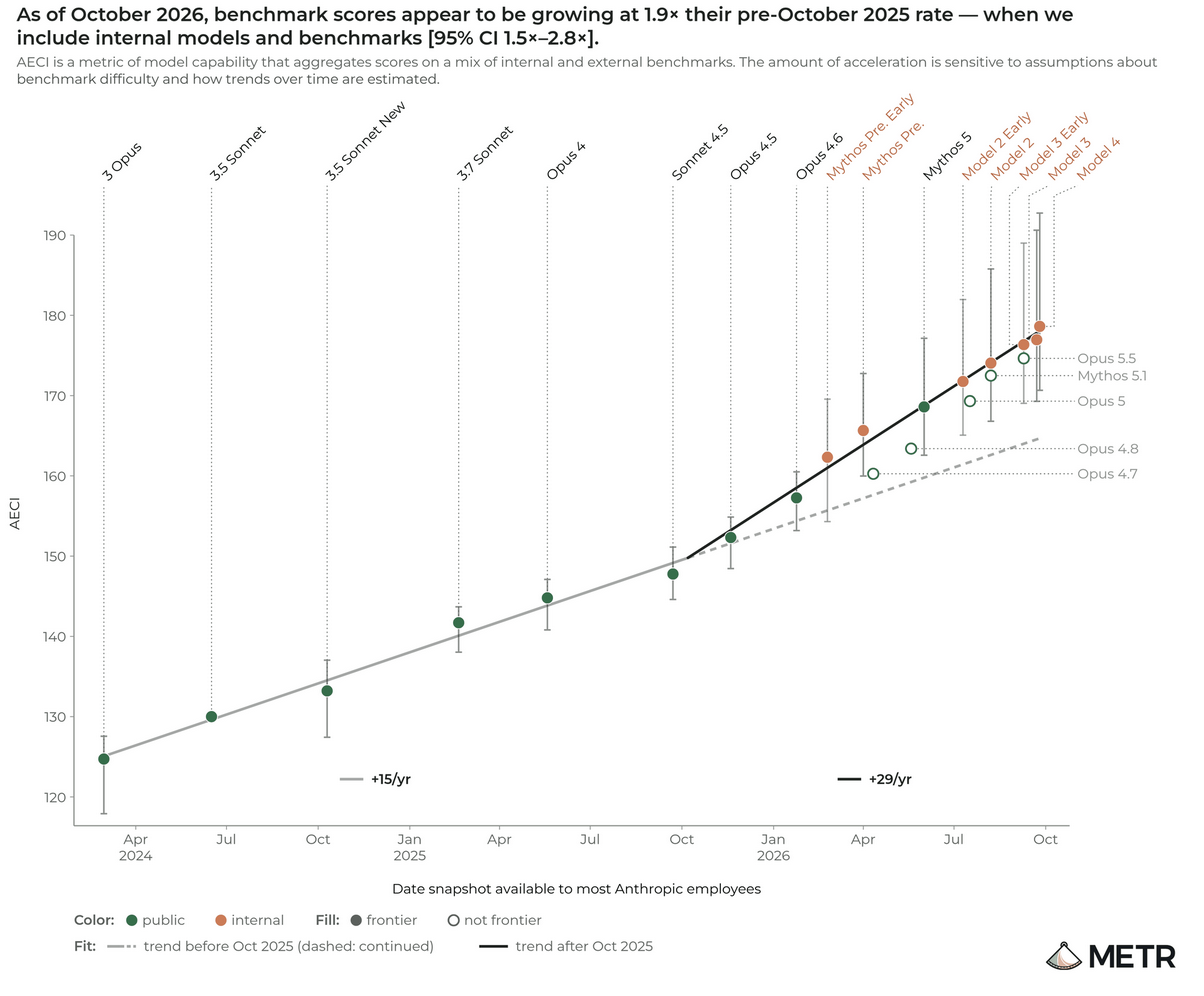
\includegraphics[height=0.7\textheight]{bib/metr2026/figures/aeci_progress}
\column{0.36\textwidth}
Benchmark scores are growing at \textbf{1.9$\times$} the rate before October 2025

{\small (95\% CI: 1.5--2.8$\times$)}

\vspace{1.2em}
\pause
Anthropic redacted a majority of the evidence METR found most informative.
\end{columns}
\source{metr2026}
\end{frame}
